        \documentclass{standalone}
        \usepackage{../BlogTikz}
        \begin{document}

  	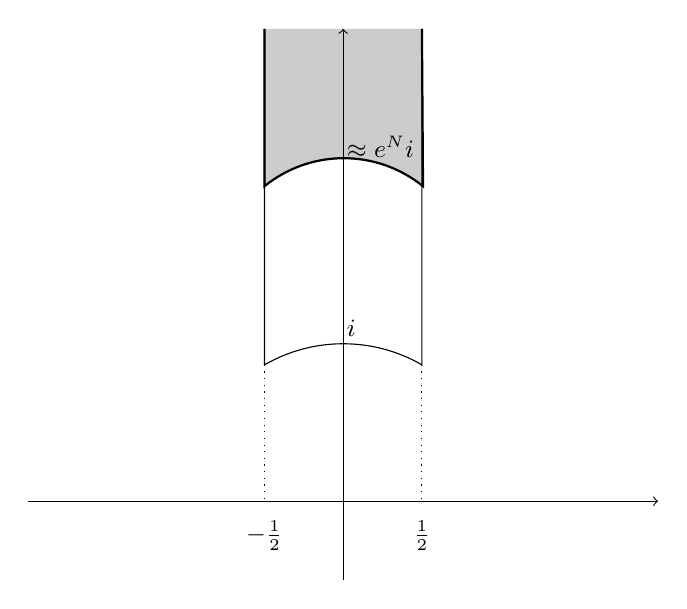
\begin{tikzpicture}[scale=2]
  	\tikzstyle{every node}=[font=\small]
  	\draw[->] (-2,0) to (2,0);
  	\draw[->] (0,-.5) to (0,3);
  	\draw (-.5,3) to (-.5,.866) arc (120:60:1) to (.5,3);
  	\draw[dotted] (-.5,.866) to (-.5,0);
  	\draw[dotted] (.5,.866) to (.5,0);
  	\node[label=below:{$\frac{1}{2}$}] at (.5,0) {};
  	\node[label=below:{$-\frac{1}{2}$}] at (-.5,0) {};
  	\node[label=right:{$i$}] at (-.1,1.1) {};
  	\filldraw[thick, fill opacity = 0.2] (-.5,3) to (-.5,2) arc (129:51:0.8) to (.5,3);
  	\node[label=right:{$\approx e^Ni$}] at (-.1,2.25) {};
  \end{tikzpicture}
          \end{document}
